%%%%%%%%%%%%%%%%%%%%%%%%%%%%%%%%%%%%%%%%%%%%%%%%%%%%%%%%%%%%%%%%%%%%%%
% LaTeX Template: Newsletter  % Source: http://www.howtotex.com
% If you're new to LaTeX, the wikibook is a great place to start:
% http://en.wikibooks.org/wiki/LaTeX
%%%%%%%%%%%%%%%%%%%%%%%%%%%%%%%%%%%%%%%%%%%%%%%%%%%%%%%%%%%%%%%%%%%%%%
% Edit the title below to update the display in My Documents
%\title{Newsletter Template}

%%% ---------------
%%% PREAMBLE
%%% ---------------
\documentclass[10pt,a4paper]{article}

% Define geometry (without using the geometry package)
\setlength\topmargin{-48pt}
\setlength\headheight{0pt}
\setlength\headsep{25pt}
\setlength\marginparwidth{-20pt}
\setlength\textwidth{7.0in}
\setlength\textheight{9.5in}
\setlength\oddsidemargin{-30pt}
\setlength\evensidemargin{-30pt}

\frenchspacing						% better looking spacing

% Call packages we'll need
\usepackage{ragged2e}
\usepackage[english]{babel}			% english
\usepackage{graphicx}				% images
\usepackage{amssymb,amsmath}		% math
\usepackage{multicol}				% three-column layout
\usepackage{url}					% clickable links
\usepackage{marvosym}				% symbols
\usepackage{wrapfig}				% wrapping text around figures
\usepackage[T1]{fontenc}			% font encoding
\usepackage{charter} 				% Charter font for main content
\usepackage{blindtext}				% dummy text
\usepackage{datetime}				% custom date
\newdateformat{mydate}{\monthname[\THEMONTH] \THEYEAR}
\usepackage[pdfpagemode=FullScreen, colorlinks=false]{hyperref}	%links and pdf behaviour

% Customize (header and) footer
\usepackage{fancyhdr}
\pagestyle{fancy}
\lfoot{	\footnotesize 
		COVID-19 Newsletter \\
		\Mundus\ \href{https://www.mohfw.gov.in}{mohfw.gov.in}	\quad
		\Telefon\ 1075											\quad
		\Letter\ \href{mailto:ncov2019@gov.in}{ncov2019@gov.in}
	  }
\cfoot{}
\rfoot{\footnotesize ~\\ Page \thepage}
\renewcommand{\headrulewidth}{0.0pt}	% no bar on top of page
\renewcommand{\footrulewidth}{0.4pt}	% bar on bottom of page

%%% ---------------
%%% DEFINITIONS
%%% ---------------

% Define separators
\newcommand{\HorRule}[1]{\noindent\rule{\linewidth}{#1}} % Creating a horizontal rule
\newcommand{\SepRule}{\noindent							 % Creating a separator
						\begin{center}
							\rule{250pt}{1pt}
						\end{center}
						}						

% Define Title en News input
\newcommand{\JournalName}[1]{%
		\begin{center}	
			\Huge \usefont{T1}{augie}{m}{n}
			#1%
		\end{center}	
		\par \normalsize \normalfont}
		
\newcommand{\JournalIssue}[1]{%
		\hfill \textsc{\mydate \today, No #1}
		\par \normalsize \normalfont}

\newcommand{\NewsItem}[1]{%
		\usefont{T1}{augie}{m}{n} 	
		\large #1 \vspace{4pt}
		\par \normalsize \normalfont}
		
\newcommand{\NewsAuthor}[1]{%
			\hfill by \textsc{#1} \vspace{4pt}
			\par \normalfont}		


%%% ---------------
%%% BEGIN DOCUMENT
%%% ---------------
\begin{document}
% Title	
% -----
\JournalIssue{1}
\JournalName{COVID-19}
\noindent\HorRule{3pt} \\[-0.75\baselineskip]
\HorRule{1pt}
% -----

% Front article
% -----

\begin{center}

    \NewsItem{What is COVID-19 ?}
    %\vspace{0cm}
	\SepRule
    \vspace{0.1cm}
	%\begin{wrapfigure}{l}{0.41\textwidth}
		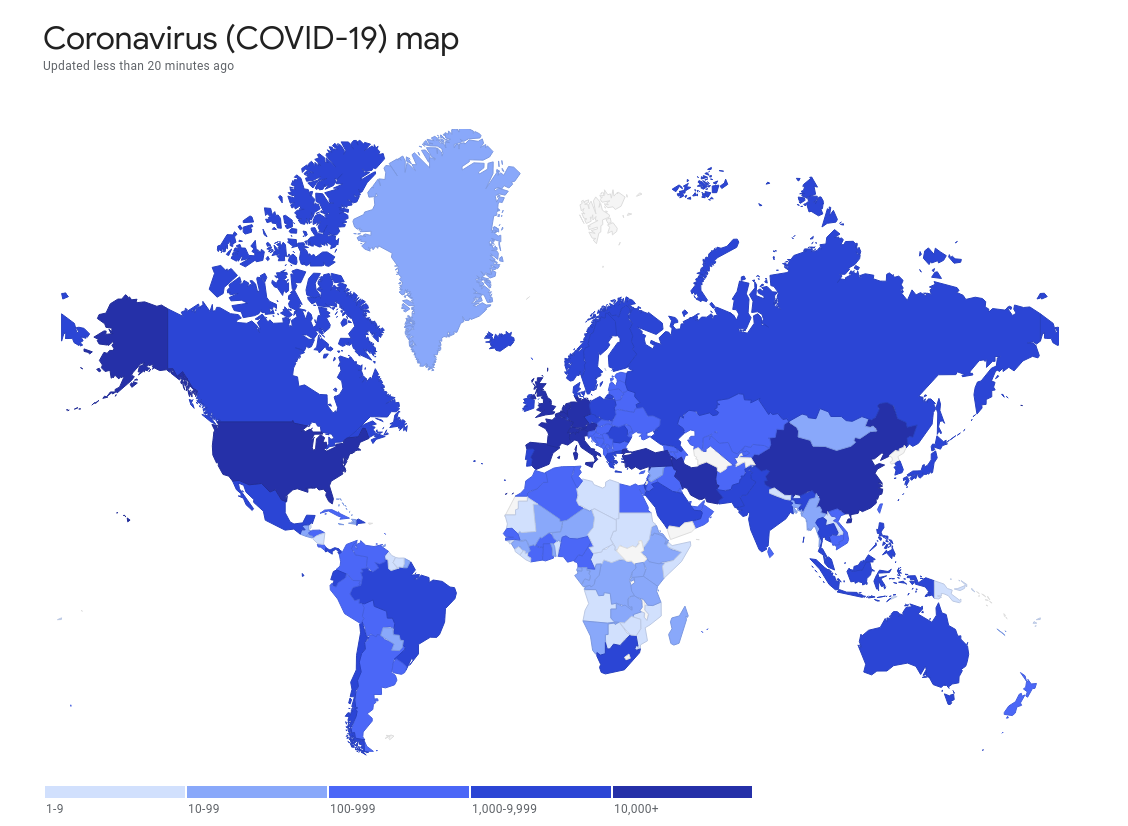
\includegraphics[width=\textwidth]{map.png}
		%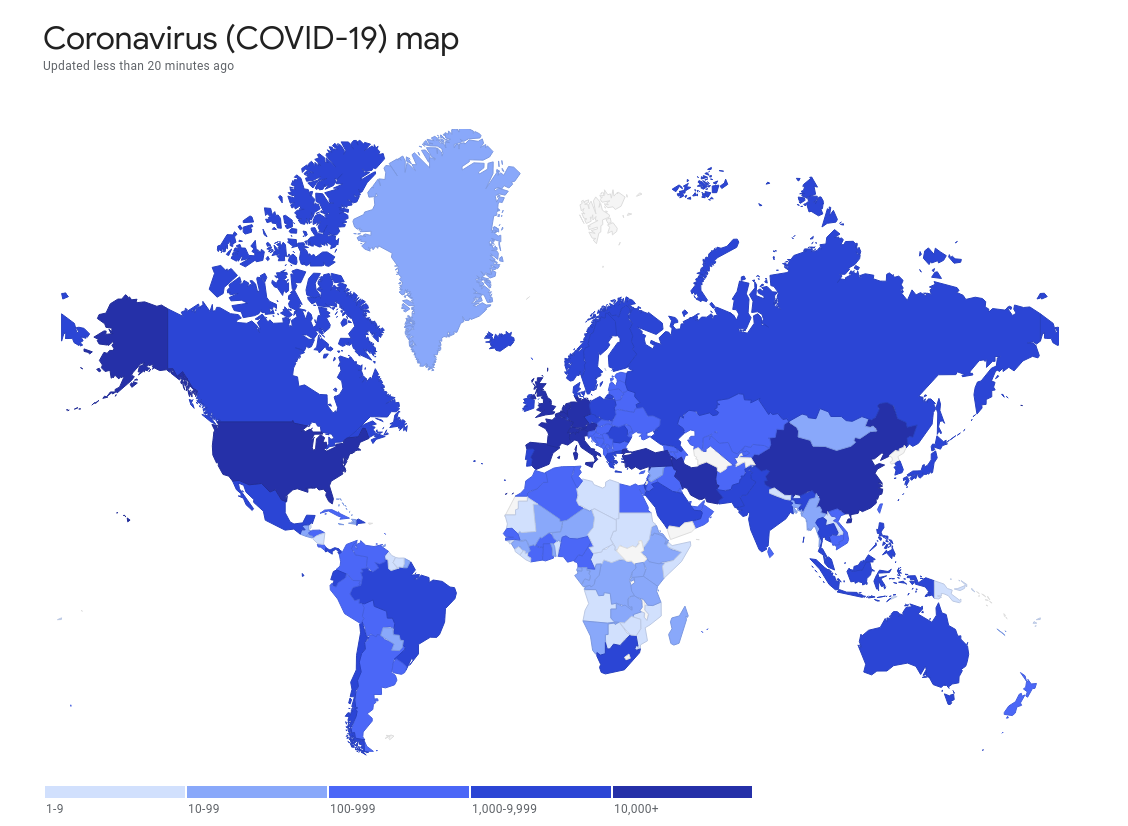
\includegraphics[]{map.png}
		\\	% this spacer is needed to make the text on the right fit OK
	%\end{wrapfigure}
	
	\textit{Coronavirus disease (COVID-19) is an infectious disease caused by a new virus. Also called: 2019-nCov, 2019 Novel Coronavirus. ICTV announced “severe acute respiratory syndrome coronavirus 2 (SARS-CoV-2)” as the name of the new virus on 11 February 2020.
	\begin{flushleft}\textbf{How does it spread ?} \end{flushleft} The COVID-19 virus spreads primarily through droplets of saliva or discharge from the nose when an infected person coughs or sneezes, so it’s important that you also practice respiratory etiquette (for example, by coughing into a flexed elbow).  It also spreads when a person touches a surface or object that has the virus on it, then touches their eyes, nose, or mouth.}
%\end{minipage}
\end{center}
% -----


% Other news (1)
% -----
\vspace{0.5cm}
	\SepRule
\vspace{0.5cm}
\begin{multicols}{2}
	\NewsItem{Symptoms}
	\NewsAuthor{W.H.O.}
	The COVID-19 virus affects different people in different ways. People may be sick with the virus for 1 to 14 days before developing symptoms. COVID-19 is a respiratory disease and most infected people will develop mild to moderate symptoms and recover without requiring special treatment.  People who have underlying medical conditions (such as asthma, diabetes, or heart disease) and those over 60 years old have a higher risk of developing severe disease and death. Common symptoms include:
	\begin{itemize}
	    \item fever
        \item tiredness
        \item dry cough.
	\end{itemize}
    Other symptoms include:
    \begin{itemize}
        \item shortness of breath
        \item aches and pains
        \item sore throat
        \item and very few people will report diarrhoea, nausea or a runny nose.
    \end{itemize}
    People with mild symptoms who are otherwise healthy should self-isolate and contact their medical provider or a COVID-19 information line for advice on testing and referral.\linebreak People with fever, cough or difficulty breathing should call their doctor and seek medical attention
% -----
\vspace{0.5cm}
	\SepRule
\vspace{0.5cm}
% Other news (2)
% -----
\NewsItem{Myth Busters}
\NewsAuthor{W.H.O.}
        \begin{itemize}
            \item Exposing yourself to the sun or to temperatures higher than 25C degrees DOES NOT prevent the coronavirus disease (COVID-19)
            \item You can recover from the coronavirus disease (COVID-19). Catching the new coronavirus DOES NOT mean you will have it for life.
            \item Being able to hold your breath for 10 seconds or more without coughing or feeling discomfort DOES NOT mean you are free from the coronavirus disease (COVID-19) or any other lung disease.
            \item Drinking alcohol does not protect you against COVID-19 and can be dangerous
            \item COVID-19 virus can be transmitted in areas with hot and humid climates
            \item Cold weather and snow CANNOT kill the new coronavirus.
            \item Taking a hot bath does not prevent the new coronavirus disease.
            \item The new coronavirus CANNOT be transmitted through mosquito bites.
            \item Hand dryers are not effective in killing the 2019-nCoV.
            \item Spraying alcohol or chlorine all over your body will not kill viruses that have already entered your body.
            \item Vaccines against pneumonia, such as pneumococcal vaccine and Haemophilus influenza type B (Hib) vaccine, do not provide protection against the new coronavirus.
            \item There is no evidence that regularly rinsing the nose with saline has protected people from infection with the new coronavirus. 
            \item There is no evidence from the current outbreak that eating garlic has protected people from the new coronavirus.
            \item People of all ages can be infected by the new coronavirus (2019-nCoV). Older people, and people with pre-existing medical conditions (such as asthma, diabetes, heart disease) appear to be more vulnerable to becoming severely ill with the virus. 
            \item  Antibiotics do not work against viruses, only bacteria.
        \end{itemize}
		
\vspace{0.5cm}
	\SepRule
\vspace{0.5cm}
\NewsItem{Statistics}
\NewsAuthor{Google}
    \begin{flushleft}\textbf{\textit{Worldwide}}\end{flushleft}
    Although the virus initially spread in China, but at the moment U.S. has the highest number of confirmed cases worldwide and Italy has the highest number of deaths worldwide. At present, the confirmed cases worldwide is a staggering 8,59,032. Below is a table showing the 5 countries with the most number of confirmed cases. Please note that this data changes rapidly, so what’s shown is probably out of date. Kindly visit  \href{https://google.com/covid19-map/?hl=en}{google.com/covid19-map} for the updated information.
    \begin{center}
        \begin{tabular}{||c c c c||}
            \hline
             Location & Confirmed & Recovered & Deaths  \\
             \hline \hline
             Worldwide & 8,59,032 & 1,78,101 & 42,322 \\
             \hline \hline
             US & 1,89,445 & 7,082 & 4,075 \\
             \hline
             Italy & 1,05,792 & 15,729 & 12,428 \\
             \hline
             Spain & 95,923 & 19,259 & 8,464 \\
             \hline
             China & 81,554 & 76,238 & 3,312 \\
             \hline
             Germany & 72,004 & 7,632 & 800 \\
             \hline
        \end{tabular}
    \end{center}
    \begin{flushleft}\textbf{\textit{India}}\end{flushleft}
    The first case in India was reported in the state of Kerala and the first casualty was reported in Kalaburagi, Karnataka. At present, Maharashtra is the state having the highest number of confirmed cases with India having a total of 1637 confirmed cases. Again, the data may not be accurate and please visit \href{https://www.mohfw.gov.in}{mohfw.gov.in} for the updated data.
    \begin{center}
        \begin{tabular}{||c c c c||}
            \hline
             Location & Confirmed & Recovered & Deaths  \\
             \hline \hline
             India & 1,637 & 133 & 38 \\
             \hline \hline
              Maharashtra & 325 & 39 & 12 \\
             \hline
              Kerala & 241 & 24 & 2 \\
             \hline
              Tamil Nadu & 124 & 6 & 1 \\
             \hline
              New Delhi & 122 & 6 & 2 \\
             \hline
              Karnataka & 105 & 8 & 3 \\
             \hline
        \end{tabular}
    \end{center}

\vspace{0.5cm}
	\SepRule
\vspace{0.5cm}
\NewsItem{Preventions}
\NewsAuthor{W.H.O.}
    There is no specific medicine to prevent or treat coronavirus disease (COVID-19). People may need supportive care to help them breathe.\linebreak If you develop a fever, cough, and have difficulty breathing, promptly seek medical care. Call in advance and tell your health provider of any recent travel or recent contact with travelers.
    \begin{center}
			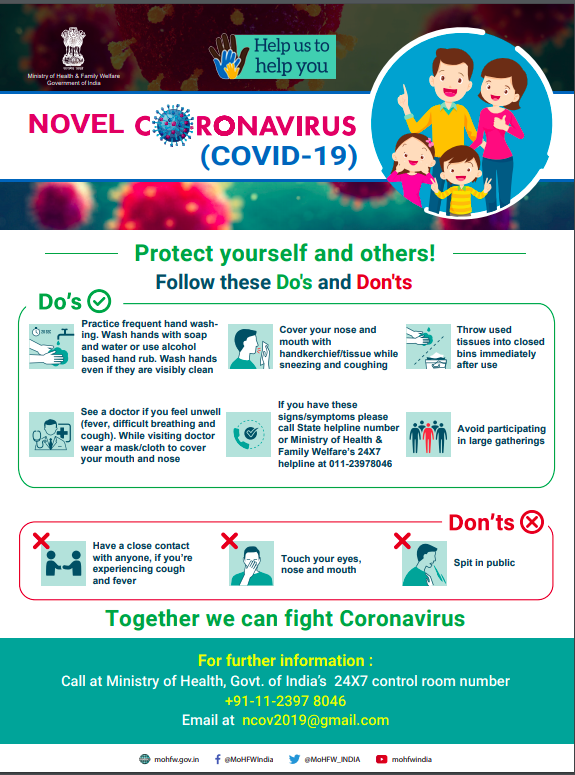
\includegraphics[width=0.4\textwidth]{dos.png}
	\end{center}
	You can protect yourself and help prevent spreading the virus to others if you:
	\begin{flushleft}\textbf{\textit{DO}}\end{flushleft}
	\begin{itemize}
	    \item Wash your hands regularly for 20 seconds, with soap and water or alcohol-based hand rub.
	    \item Cover your nose and mouth with a disposable tissue or flexed elbow when you cough or sneeze.
	    \item Maintain at least 1 metre distance between you and people coughing or sneezing.
	    \item Stay home and self-isolate from others in the household if you feel unwell.
	    \item Practice physical distancing by avoiding unnecessary travel and staying away from large groups of people.
	    
	\end{itemize}
	\begin{flushleft}\textbf{\textit{DONT}}\end{flushleft}
	\begin{itemize}
	    \item Touch your eyes, nose, or mouth if your hands are not clean
	    \item Smoke and other activities that weaken the lungs.
	    \item Spit in public.
	\end{itemize}

\end{multicols}

%\vspace{0.1cm}
	\SepRule
%\vspace{0.1cm}
\begin{center}
\NewsItem{Stay Safe, Stay Hydrated \& Keep Breathing}
\NewsAuthor{Sudhanshu Kumar}
\end{center}

% -----
\end{document} 
